%% Autor: Björn Ritterbecks 
%% Letzte Aenderung: 15.06.2016 
\thisfloatsetup{%
  capbesidewidth=\marginparwidth}
\begin{figure}[htbp]
\vspace*{0.2cm}
\centering
%\sansmath
 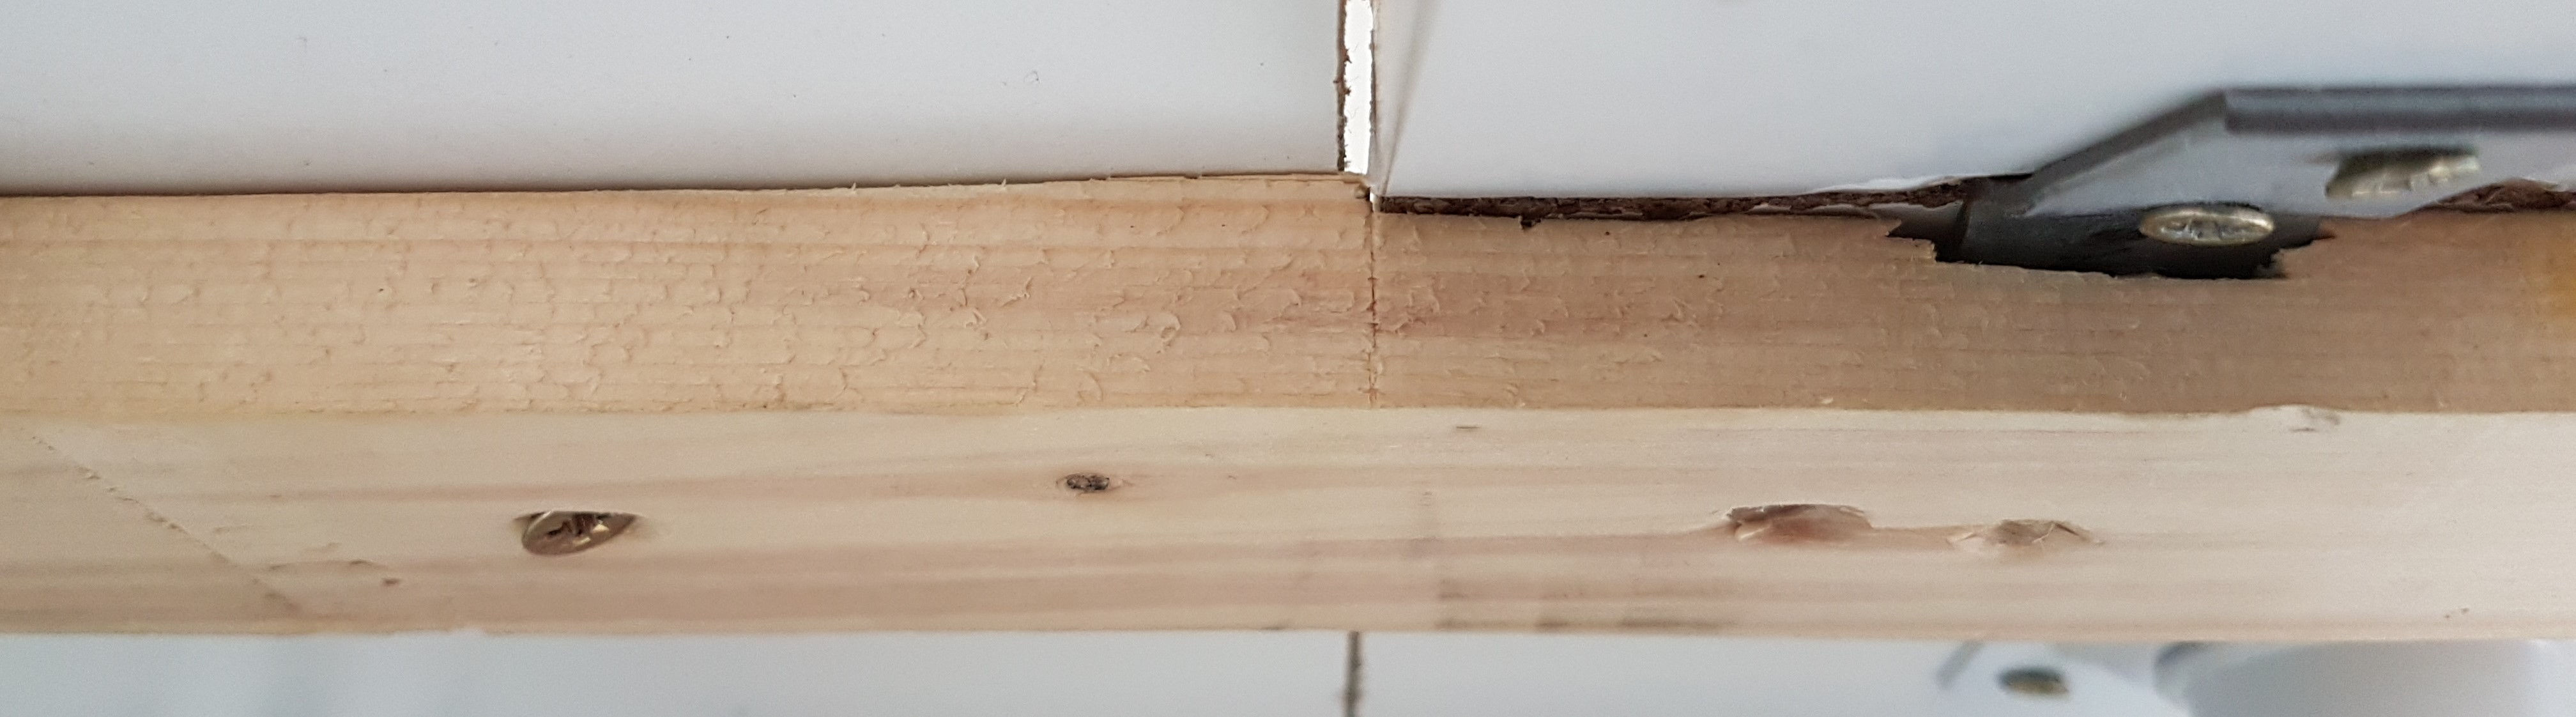
\includegraphics[width=0.99\textwidth]{images/brettvorderplatte.jpg}
  \caption[Übergangsbereich schiefe Ebene]{Zu sehen ist der Übergangsbereich zwischen schiefer Ebene und waagerechter Platte, der jeweils an der Vorder- und Hinterkante mit einem passend abgehobeltem Brett fixiert wird. Der um $\SI{15}{\degree}$ geneigte Plattenteil ist erst nach den Messungen hinzugefügt worden, um der Winkelaufspaltung der Kugeln genüge zu tun (d.\,h., dass die Breiten der einzelnen Detektoren nach rechts hin zunehmen müssen.)}
  \label{fig:brettvorderplatte}
  \vspace{-0pt}
\end{figure}